\chapter{Problemanalyse}
    \label{chapter:ProblemAnalysis}
    \section{\imperia}
    \section{\wordpress}
    \section{Klassifizierung der Inhalte einer Webseite}
        %\url{http://www.fernuni-hagen.de/KSW/portale/babw/service/}

        %\begin{figure}
        %    \centering
        %    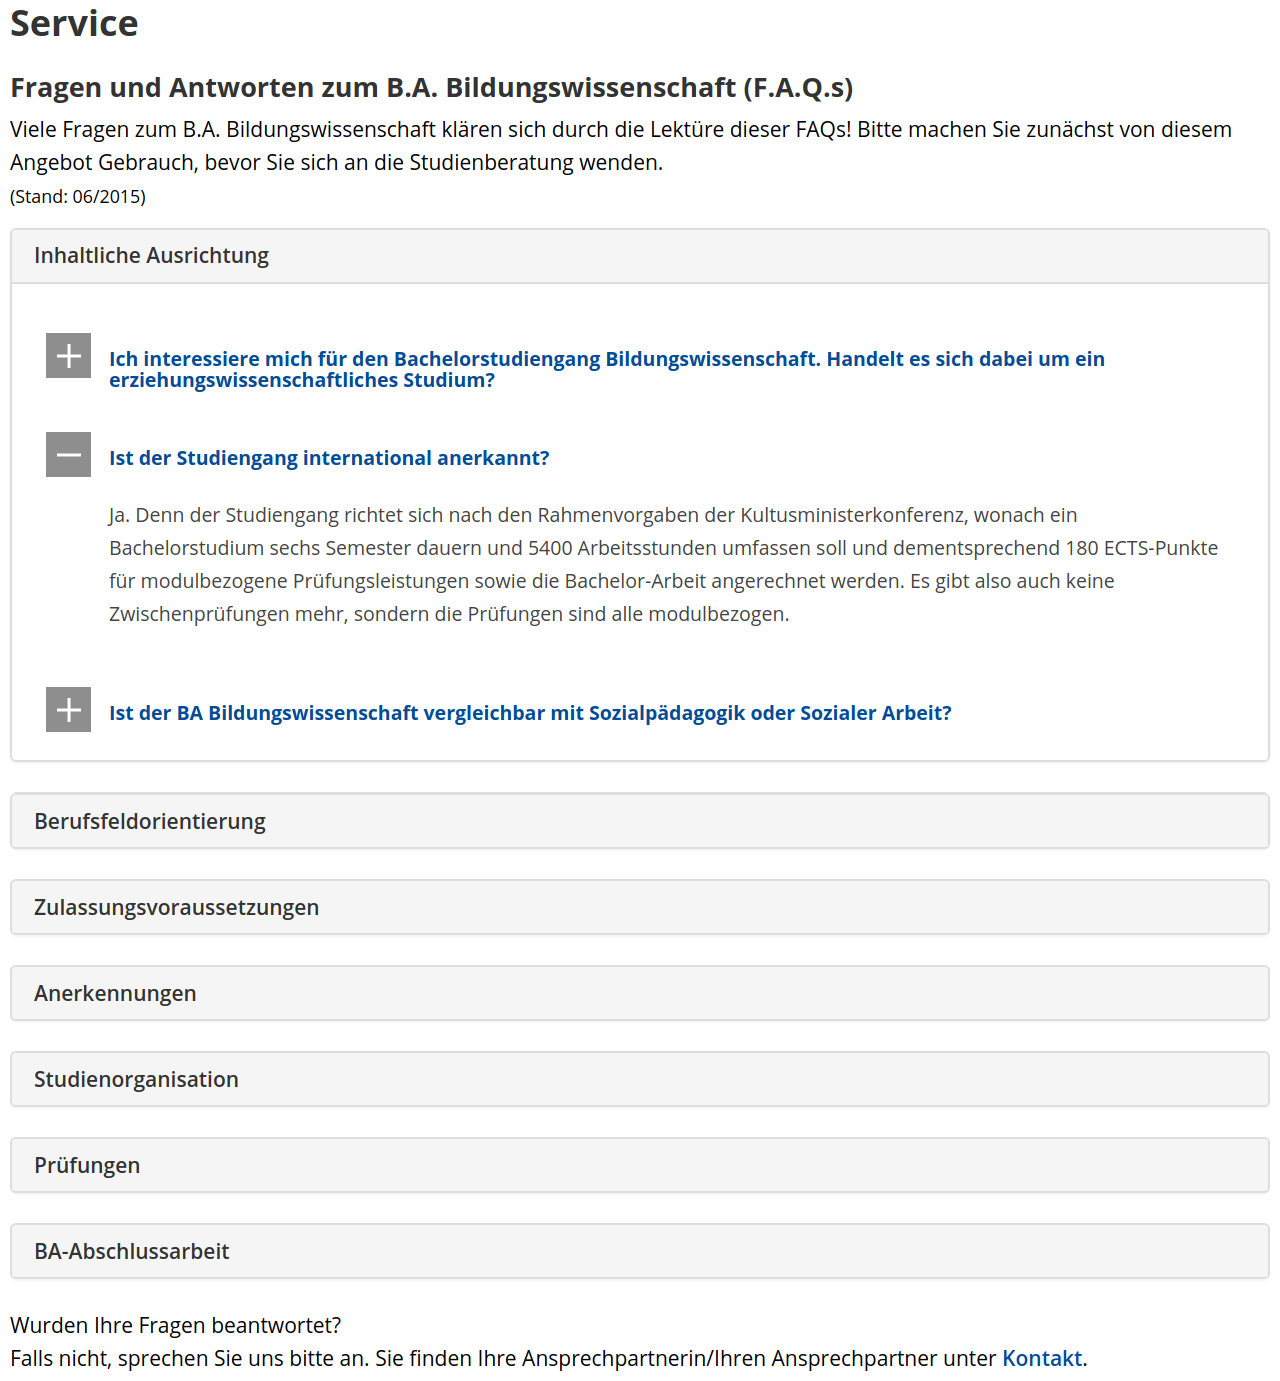
\includegraphics[width=\textwidth]{../resources/babw_service_faq.png}
        %    \caption{FAQ Seite des Studienportals B.A. Bildungswissenschaft}
        %    \label{image:BuildingBlocks}
        %\end{figure}
    
    \section{Das World Wide Web}
        Zur Lösung der beschriebenen Problemstellung ist eine genauere
        Betrachtung ihrer Domäne notwendig.
        Das Problem wird dadurch in einen größeren Kontext gesetzt,
        was zu einem besseren Verständnis und damit zur Findung
        einer geeigneten Lösung beiträgt.
        % TODO: Ref auf DDD?

        Die in diesem Fall zu betrachtende Domäne ist das "`\gls{www}"',
        welche das \gls{w3c} wie folgt definiert \cite{w3c:wwwArch}:

        \begin{quote}
            The \textit{\textbf{World Wide Web}} (\textit{\textbf{WWW}}, or simply \textit{\textbf{Web}})
            is an information space in which the items of interest, referred to as resources,
            are identified by global identifiers called Uniform Resource Identifiers (\textit{\textbf{URI}}).
        \end{quote}

        Diese Problemdomäne wird im Folgenden aus zwei Perspektiven betrachtet:
        Zunächst wird die Sicht eines Webseitenbesuchers auf das \gls{www} beschrieben.
        Anschließend stehen die konzeptionellen und technischen Grundlagen
        des \gls{www} im Vordergrund.
        Zusammen vermitteln diese Erläuterungen hinreichendes Wissen,
        um eine Lösung für die gegebene Problemstellung zu erarbeiten.

        \subsection{Das World Wide Web für Webseitenbesucher}
            Die Sicht eines Webseitenbesuchers (im Folgenden auch "`Endnutzer"' genannt)
            auf das \gls{www} ist simpel und sollte von jedem Leser nachvollzogen werden können.
            Dennoch bietet sie wichtige Einblicke.

            \paragraph*{Der Browser}
            Zugang zum \gls{www} erhält ein typischer Endnutzer über einen \textit{Browser}.
            In dessen Adresszeile trägt er einen \gls{url} ein,
            woraufhin der Browser die gewünschte Webseite lädt und anzeigt.
            Eine Webseite ist aus Sicht eines Endnutzers also eindeutig über eine
            Adresse, die allgemein "`URL"' oder "`Link"' genannt wird, gekennzeichnet.
            Der Browser dient zur Anzeige von Webseiten, wodurch er für Webseitenbesucher
            zu einem unentbehrlichen Werkzeug wird.
            Browser existieren für verschiedene Endgeräte,
            wie PCs, Smartphones und Tablets.
            Das heißt ein Webseitenbesucher ist an eine Form von Endgeräten gebunden.

            \paragraph*{Bestandteile}
            Sieht sich ein Besucher eine Webseite im Browser an,
            kann er schnell verschiedene Bestandteile ausmachen.
            Dazu zählen zunächst simple Elemente, mit denen er wenig bis gar nicht
            interagieren kann, also statischer Natur sind.
            Vertreter dieser Gruppe sind

            \begin{itemize}
                \item Texte,
                \item Bilder,
                \item Videos,
                \item Links auf andere Webseiten und
                \item Dateien, die zum Download bereitstehen.
            \end{itemize}

            Des Weiteren besitzt eine Webseite Designelemente,
            die in ihrem Aufbau oder ihrer Funktion komplexer
            als die zuvor genannten sind.
            Die Bibliothek Bootstrap\footnote{https://getbootstrap.com/}
            enthält zahlreiche solcher Komponenten.
            Beispielsweise bietet die Komponente "`Card"' die Möglichkeit
            Inhalte in komplexe Behälter einzubetten \cite{bootstrap:Cards}.
            Ein anderes Beispiel ist die Komponente "`Carousel"',
            welche der Erstellung von Diashows dient \cite{bootstrap:Carousel}.
            Letztere und viele weitere bieten dem Nutzer
            erweiterte Möglichkeiten zur Interaktion mit einer Webseite.

            Das gilt auch für Formular- oder Steuerelemente,
            die aus klassischen Applikationen bekannt sind,
            aber auch in Webseiten Anwendung finden.
            Dazu gehören unter anderem

            \begin{itemize}
                \item Textfelder,
                \item Schaltflächen,
                \item Dropdown-Listen,
                \item Checkboxen und
                \item Radiobuttons.
            \end{itemize}

            Allen Elementen ist gemein, dass ihr Aussehen sich von
            zwischen verschiedenen Webseiten unterscheiden kann.

            \paragraph{Varianten}
            Aus Sicht eines Endnutzers existieren oftmals mehrere
            Varianten derselben Webseite.
            Welche Variante er sieht hängt dabei von zwei Dimensionen ab:
            Sprache und Endgerät.

            Die heutige globalisierte und vernetzte Welt machen es oft erforderlich
            einen Internetauftritt auch auf internationele Besucher vorzubereiten.
            An erster Stelle bedeutet dies, dass Inhalte in verschiedene Sprachen
            übersetzt werden, um sie einem möglichst großen Publikum zugänglich zu machen.
            Für einen Endnutzer gibt es prinzipiell zwei Methoden,
            wie er eine Seite in seiner favorisierten Sprache anzeigen kann:

            \begin{itemize}
                \item   Die Webseite bietet ihm ein Steuerelement,
                        über das er selbst eine Sprache auswählen kann.
                \item   Die Webseite ermittelt automatisch die geeignete Sprache,
                        anhand verschiedener Parameter, die für den Besucher nicht zwangsläufig
                        offensichtlich sind.
            \end{itemize}

            Die Popularität mobiler Endgeräte wie Smartphones und Tablets
            bewegt immer mehr Betreiber von Webseiten dazu,
            verschiedene Versionen ihres Internetauftrittes anzubieten,
            die für verschiedene Geräte optimiert sind.
            Aus Sicht eines Besuchers gibt es bis zu drei geräteabhängige
            Varianten einer Webseite. Zwei für die oben genannten mobilen Geräte
            sowie eine weitere für PCs.
            Für ihn sind dabei drei Unterscheidungsmerkmale dieser Varianten offensichtlich:

            \begin{enumerate}
                \item Inhalt,
                \item Design und
                \item Funktionalität.
            \end{enumerate}

        \subsection{Konzeptionelle und technische Grundlagen}